\documentclass[12pt,letterpaper]{article}
\usepackage{amsmath,amsthm,amsfonts,amssymb,amscd}
\usepackage{fullpage}
\usepackage{lastpage}
\usepackage{enumerate}
\usepackage{fancyhdr}
\usepackage{mathrsfs}
\usepackage{xcolor}
\usepackage{graphicx}
\usepackage{algorithm2e}
\usepackage[margin=3cm]{geometry}
\setlength{\parindent}{0.0in}
\setlength{\parskip}{0.05in}

% Edit these as appropriate
\newcommand\course{CS 476/676}
\newcommand\semester{Fall 2013}     % <-- current semester
\newcommand\hwnum{1b}                  % <-- homework number
\newcommand\yourname{David Snyder} % <-- your name
\newcommand\login{Hopkins ID: dsnyde29}       
\newcommand\hwdate{Due: October 22rd 2013}           % <-- HW due date

\newenvironment{answer}[1]{
  \subsubsection*{Problem #1}
}


\pagestyle{fancyplain}
\headheight 35pt
\lhead{\yourname\ \login\\\course\ --- \semester}
\chead{\textbf{\Large Homework \hwnum}}
\rhead{\hwdate}
\headsep 10pt

\begin{document}

\noindent \emph{Homework Notes:} Notes \\

\begin{answer}{2.1.1}

\begin{figure}[h!]
  \caption{Drawing of $\mathcal{F}'$.}
  \centering
    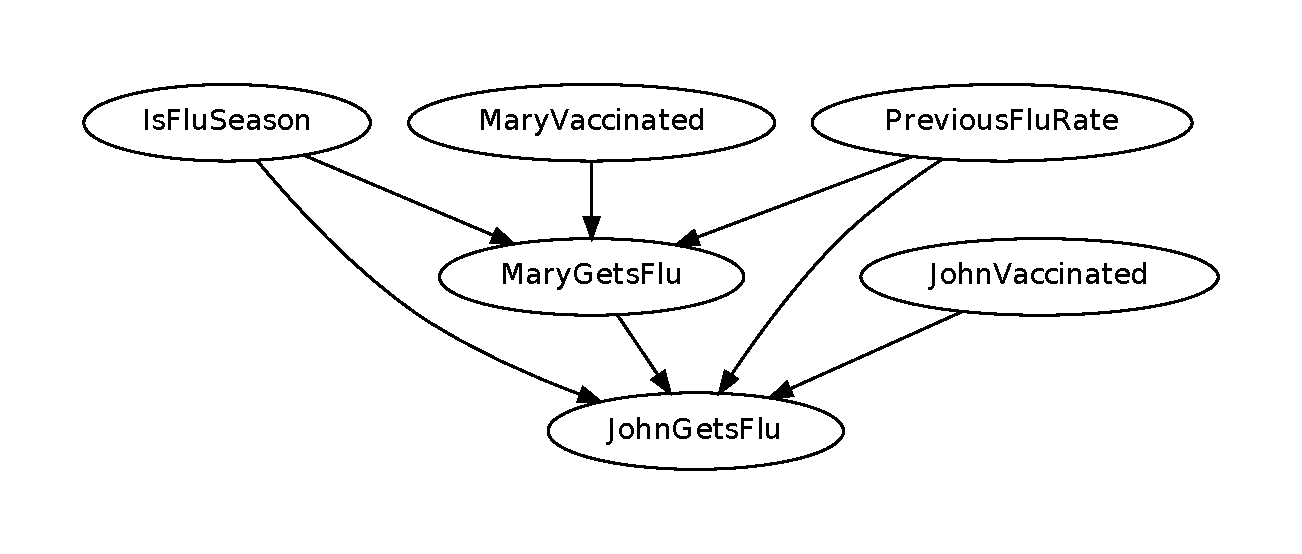
\includegraphics[width=1\textwidth]{graph.pdf}
\end{figure}

\end{answer}

\begin{answer}{2.1.2}

The procedure used to produce the drawing above is as follows.
List all of the independencies in $\mathcal{F}$. Remove any independence which
includes FluRate. Now, the remaining independencies guide our creation of
$G'$. 

\begin{algorithm}[H]
 %\SetAlgoLined
 \KwData{Bayesian network $\mathcal{F}'$ and a node to remove $X$}
 \KwResult{Bayesian network $\mathcal{F}'$ such that $X$ is eliminated}
 initialization\;
 $\mathcal{F}' = \{\}$\;
 \For{$i$ in $Imap(\mathcal{F})$}{
  \eIf{$X$ not in $i$}{
   $Imap(\mathcal{F}') \leftarrow Imap(\mathcal{F}') \cup \{i\}$\;
   }{
  }
 }
 \For{Nodes $n$ and $m$ \in $Z$ }{
   \eIf{not $dsep(n;m \mid Z)$ }{
     \eIf{ $\exists g \in G$ such that $g = edge(n,m)$ or $g = edge(m,n)$ }{
       $edges(G') \leftarrow edges(G') \cup \{g\}$\;
     }
     \eElse{}{
       $edges(G') \leftarrow edges(G') \cup \{(n,m)\}$\;
     }
   }
 }
\end{algorithm}


\end{answer}

\begin{answer}{2.2.1.1}

Suppose that there is no active trail from $\hat{Z}$ to $X$ and there exists some $B_1$ and $B_2$ 
such that $P_{B_{1}}(X \mid Y) \ne P_{B_{2}}(X \mid Y)$.
Since there is no active trail between $\hat{Z}$ and $X$, by properties of d-separation,
we can conclude that $dsep(X ; \hat{Z} \mid Y)$. It must be the case that $P_{B_{1}}(X \mid Y) \ne P_{B_{2}}(X \mid Y)$
due to some node $N$ on an active trail $U$ to $X$ given $Y$.
There are two possibilities, either $N$ is also on an active trail with $\hat{Z}$ or the CPD of $N_{B_{1}}$ and $N_{B_{2}}$ are different even though $dsep(N ; \hat{Z} | Y)$. The first case is false since if $N$ were on an active trail with $\hat{Z}$, then $X$ would also be on $U$, but there is no
active trail from $\hat{Z}$ to $X$. The second case is also false, since by definition of $B_{1}$ and $B_{2}$, the CPDs of $N_{B_{1}}$ and $N_{B_{2}}$are identical.
But this contradicts our assumption, so it must be the case that if there is no active trail from $\hat{Z}$ to
$X$ then for all $B_{1}$ and $B_{2}$ $P_{B_{1}}(X \mid Y) = P_{B_{2}}(X \mid Y)$. 

\end{answer}

\begin{answer}{2.2.1.2}

Suppose not. Suppose that Z is a requisite node for P(X|Y) and Pb1(X|Y) = Pb2(X|Y) for all B1 and B2. Let B1 and B2 be some particular B1 and B2
such that G consists of the following topology Zhat -> Z -> X <- Y so that there is an active trail from Zhat to X given Y as required by the fact that Z is a requisite node for P(X|Y). 
Let all CPDs be nonzero
for all values of the random variables. Further, let Zhat B1 SOME RELATIONSHIP  with Zhat B2 STUFF HAPPENS so we see that pb1(X|Y) not equal pb2(X|Y). This contradiction allows us to negate our premise. We can then conclude that if Z is a requisite node for P(X|Y) then pb1(X|Y) = pb1(X|Y) for all
B1 and B2. 
\end{answer}

\begin{answer}{2.2.3.1.a}

Let $MB_{G}(X)$ denote the Markov blanet of a node $X$ in an undirected graph $G$, whose set of nodes is denoted $\mathcal{X}$. We will show that
for any $X$ such that $W = \mathcal{X} - \{X\} - MB_{G}(X)$ then $X$ and $W$ are separated given $MB_{G}(X)$. 
\\
Suppose that $X$ and $W$ are not separated given $MB_{G}(X)$. That is, \neg $sep(X;Y \mid MB_{G}(X))$. Then there is some path $U$ from a node $N \in W$to $X$, given $MB_{G}(X)$. Since this path exists, there must be some $M \in U$ such that $M$ is a neighbor of $X$. However, by definition of the
Markov Blanket, $M \in MB_{G}(X)$. Thus, it cannot be that $M \in U$, and this extends to all possible $M$. But then, $U$ cannot exist and so by
Contradiction, the negation of our premise must be true, that is, $X$ and $W$ are separated given $MB_{G}(X)$.


\begin{answer}{2.2.3.1.b}
Let $MB_{G}(X)$ denote the Markov blanet of a node $X$ in an undirected graph $G$, whose set of nodes is denoted $\mathcal{X}$. We will show that
for any $X$ such that $W = \mathcal{X} - \{X\} - MB_{G}(X)$ then $X$ and $W$ are separated given $MB_{G}(X)$ and $MB_{G}(X)$ is the minimal set
with this property.
\\
Suppose that $MB_{G}(X)$ is not minimal. Then there exists some neighbor of $X$ $N \in \mathcal{X}$ such that $MB_{G}'(X) = MB_{G} - \{N\}$ separates $X$ and $W$,
that is, $sep(X;W \mid MB_{G}'(X))$. Let $M \in W$ be some node such that there is a path $U$ shared by $M$ and $N$. Then it must be that $X \in U$,
since $N$ is a neighbor of $X$. Because such a path exists, $\neq sep(X;M \mid MB_{G}'(X))$, which contradicts our supposition. Therefore, $MB_{G}(X)$ must be the minimal set with this property.
\end{answer}

\begin{answer}{2.2.3.2}

Let $B$ be a Bayesian network with a graph $G$.
By Definition 4.16 Corollary 4.2, we can create an undirected moral graph from $G$ denoted $M[G]$, such that it is an I-map for $P_{B}$. Therefore,
we can show the Markov blanket separates a node $X \in B$ from the remaining nodes and that this set is minimal by first converting $B$ into $M[G]$ and repeating the proofs 2.2.3.1.a and 2.2.3.1.b on the resultant Markov network. 

\end{answer}

\begin{answer}{2.4.1.a}

\begin{description}
\item[HMM] Yes. Influence can flow from $S_{3,1}$ to
$Y_{1}$. We can examine each overlapping triplet of
nodes and apply the rules for an active trail. Since there is an active trail, it is indeed possible for
$P(Y_{1} = severe | S_{3,1} = yes) \le P(Y_{1} = severe | S_{3,1} = no) $.
\item [MEMM] No. Again, we examine the potential active
trails. We see that due to the v-structure at $Y_{3}$
and the fact that $Y_{3}$ is not observed, influence
cannot flow to $Y_{1}$. As a result, $P(Y_{1} = severe | S_{3,1} = yes) = P(Y_{1} = severe | S_{3,1} = no) $
\item[CRF] Yes. Influence can flow $S_{3,1}$ to
$Y_{1}$ over the undirected edges and so $P(Y_{1} = severe | S_{3,1} = yes) \le P(Y_{1} = severe | S_{3,1} = no) $
\end{description} is possible.

\end{answer}

\begin{answer}{2.4.1.b}

\begin{description}
\item[HMM] No. This is a causal trail from $Y_{2}$ to
$S_{3,1}$ which is made d-separated by observing $Y_{3}$.
\item [MEMM] Yes. In the v-structure at $S_{3,1} \leftarrow Y_{3} \rightarrow Y_{2}$ influence can flow from
$S_{3,1}$ to $Y_{2}$ since $Y_{3}$ is now observed.
\item[CRF] No. The active trail is broken by observing
$Y_{3}$.

\end{answer}

\begin{answer}{2.4.1.c}

In all of the graphs, $S_{3,1}$ becomes d-separated or
separated from $Y_{1}$ given $Y_{2}$. This is evident
from the properties of Causal trails in directed graphs,
and separation in undirected graphs.

\end{answer}

\begin{answer}{2.4.2.a}

\begin{description}
\item[HMM] Because of the causal direction of the arrows from $Y$ to $S$, we can naturally compute $P(S \mid Y)$. To compute $P(Y \mid S)$ we need to be able to obtain $P(S)$ and $P(Y)$
that give us the probability of the symptoms and
the disease respectively. If we are experts in Biology
then we should be able to construct reasonable models
for $P(Y)$ and $P(S)$, making the HMM efficient for
situations in which we don't have much data. If we 
don't have good priors, then we may be better off using
one of the other models.
\item [MEMM] In this model we can more naturally compute
$P(Y | S)$. Since we have causality from the features
$S$ to the disease state $Y$ it seems easier to handle
large numbers of features. Also, in this model the features are allowed to be dependent given the disease label. This could allow for more flexibile features, such as overlapping features.
\item[CRF] It seems that this model has the same advantages as MEMM regarding flexible features. In addition, as observed in the previous questions, it allows for long range dependencies of features through time. 
\end{answer}

\begin{answer}{2.4.2.b}
As discussed above, it seems that MEMM and CRFs are better at handling correlated symptom variables (and CRFs are superior to MEMMs at correlated symptoms over time).
\end{answer}

\begin{answer}{2.4.3.b}
Suppose not, suppose that $P(x^{1} \mid z^{1}) \le P(x^{1} \mid y^{1}, z^{1})$. 
\begin{answer}{2.4.3.b}

\item
\begin{tabular}{c|c c c c}
$Z$ & $x^0,y^0$ & $x^0,y^1$ & $x^1,y^0$ & $x^1,y^1$ \\ \hline
$z^0$ & .1 & .8 & .8 & .1 \\
$z^1$ & .9 & .2 & .2 & .9
\end{tabular} \\


\begin{answer}{2.4.3.c}
$Z$ is in dependent of $Y$ in the context of $X = x^{1}$. $Z$ is also independent of $X$ in the context of $Y = y^{1}$.
\end{answer}

\end{document}
